
\clearpage
\section{Results and Discussions}

\subsection{User Interface Representation}
We have made a website for showing the project working.
\subsubsection{Brief Description of Various Modules of the system}
Class of Blockchain having many functions:
\begin{itemize}
    \item Create Blockchain: Returning a block which is the having all information about it.
    \item get previous block: It will return hash of previous block.
    % \item proof of authority: It will authorise the user.
    \item hash: Return sha256 hash of encoded block.
    \item is\_chain\_valid: It will return True if the chain is valid else False.
    \item file\_to\_sha256: It will convert file into hash and return hash value of document.
    \item encrypt\_file: This function will encrypt our file using private key of particular user and return encrypted file and key.
    \item decrypt\_file: This function will decrypt the file using private key of particular user and write decrypted content int the file placed that we will pass through function.
    \item save\_chain: This function will save chain in the database so that it will be accessible when we rerun our project.
    \item is\_document\_valid: It will return true if document is valid else false.
    % \item 
\end{itemize}

\subsection{Snapshots of system with brief detail of each}
The website includes many pages 

\begin{itemize}
    \item Dashboard page It includes showing certificates of particular user.  There is also a option through user can preview his/her certificate and even he/she can download it. There is also hash of particular user from where one can copy.
    
    \item User can login using username and password and then after checking password from the back-end, if it's correct then he/she can be redirected to the dashboard page.
    
    \item Add User: Admin can add the student using student's name, CRN and email. 
    
    \item Upload Certificate: Admin can upload username's certificate through block-chain in a securely manner.
    
    \item Admin Page: On this page, admin can select option between Add User, Upload Certificates, Get chain, Is Chain Valid.
    
\end{itemize}

\begin{figure}[h]
    \centering
    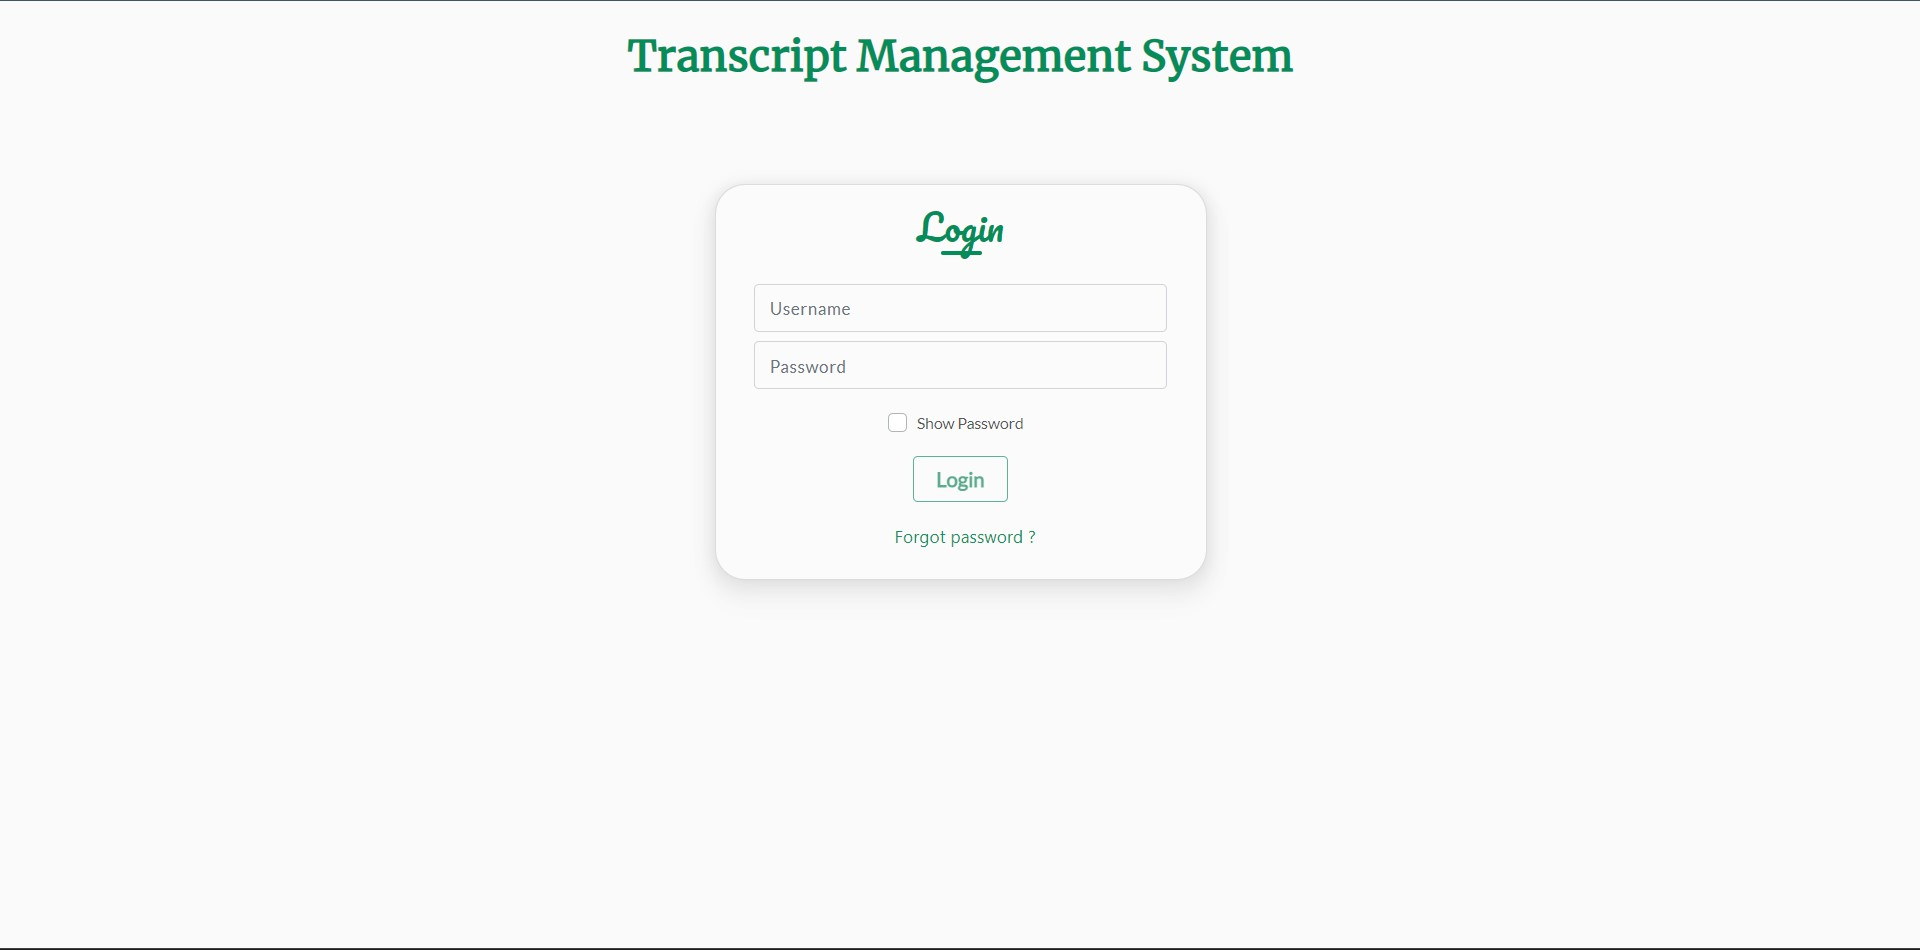
\includegraphics[scale=0.32]{images/login.jpg}\\[0.5cm]
    \caption{Login Page}
    \label{fig:login}
\end{figure}

\begin{figure}[H]
    \centering
    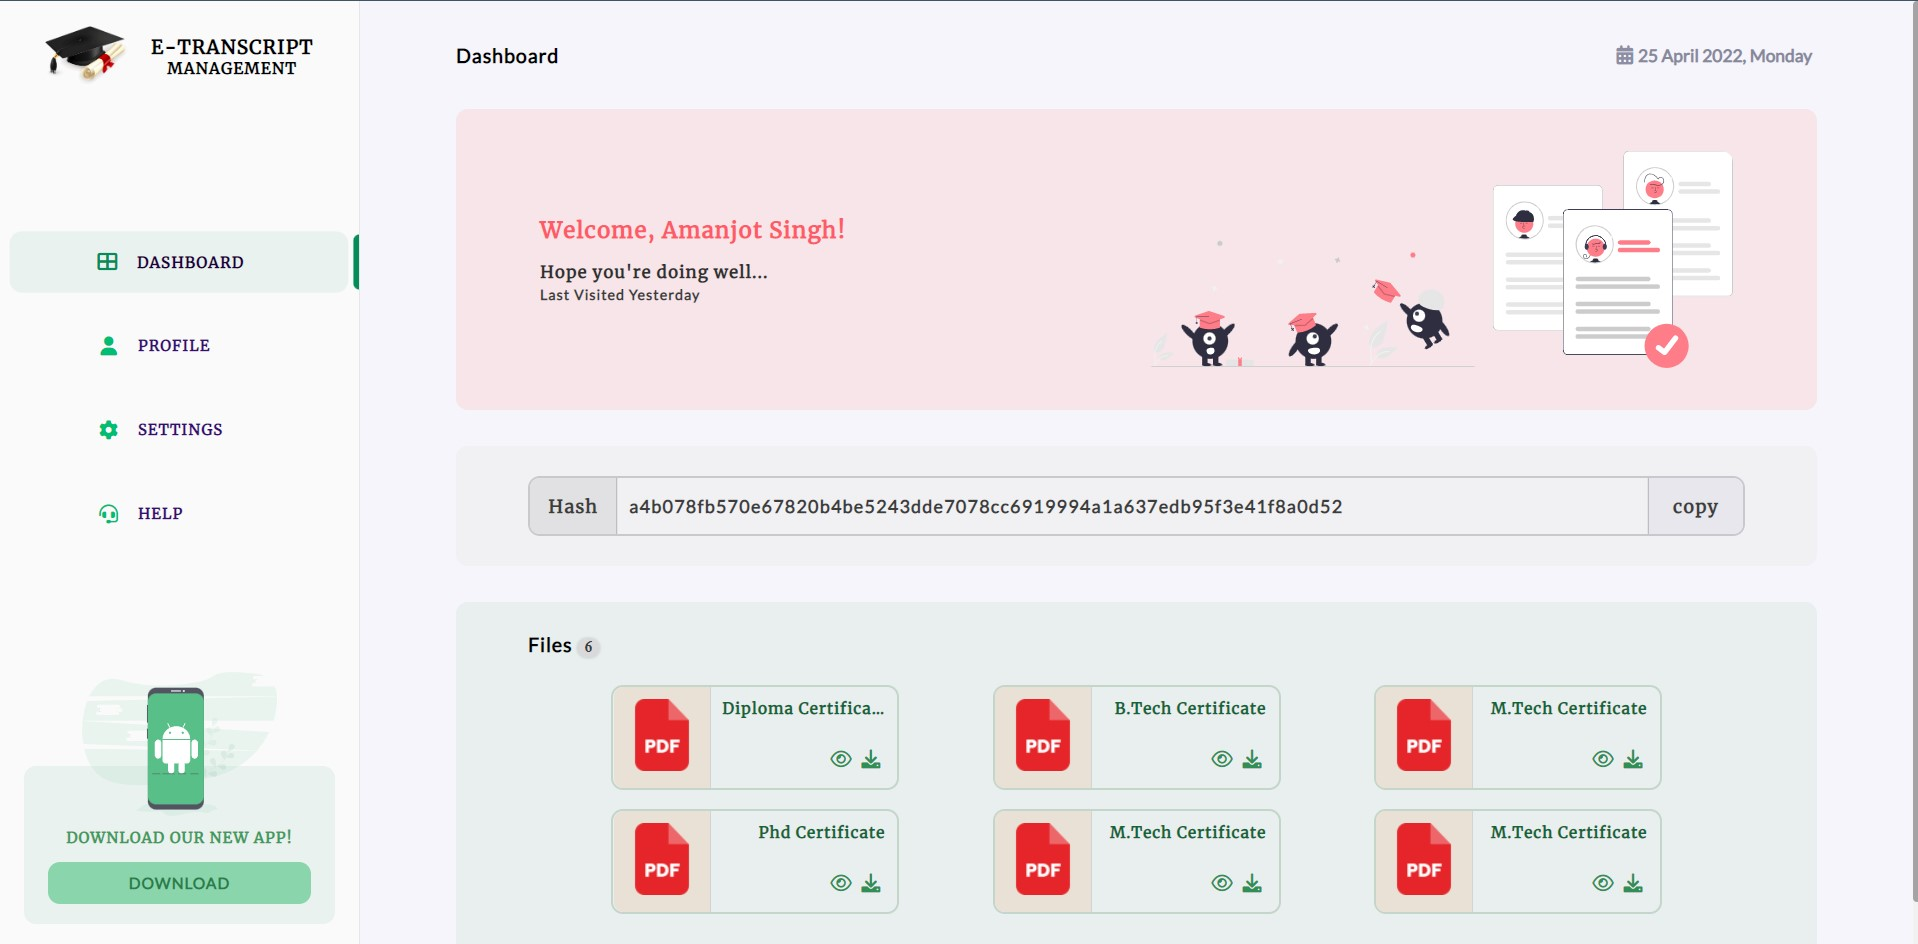
\includegraphics[scale=0.32]{images/Dashboard.jpg}\\[0.5cm]
    \caption{Dashboard Design}
    \label{fig:my_label}
\end{figure}

\begin{figure}[H]
    \centering
    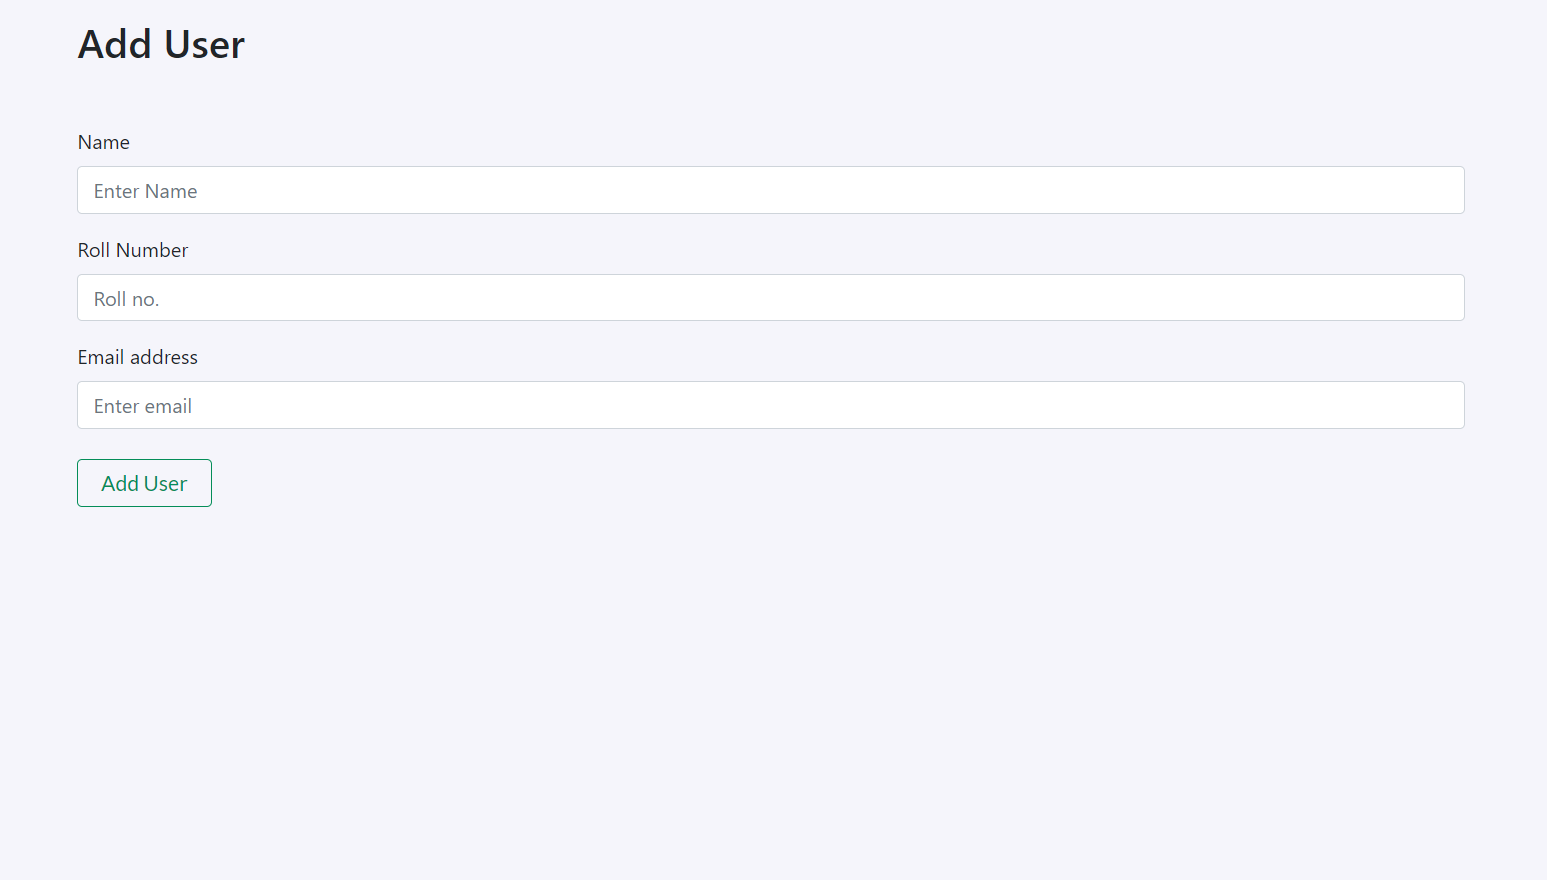
\includegraphics[scale=0.4]{images/add_user.png}\\[0.5cm]
    \caption{Add User Design}
    \label{fig:my_label}
\end{figure}

\begin{figure}[H]
    \centering
    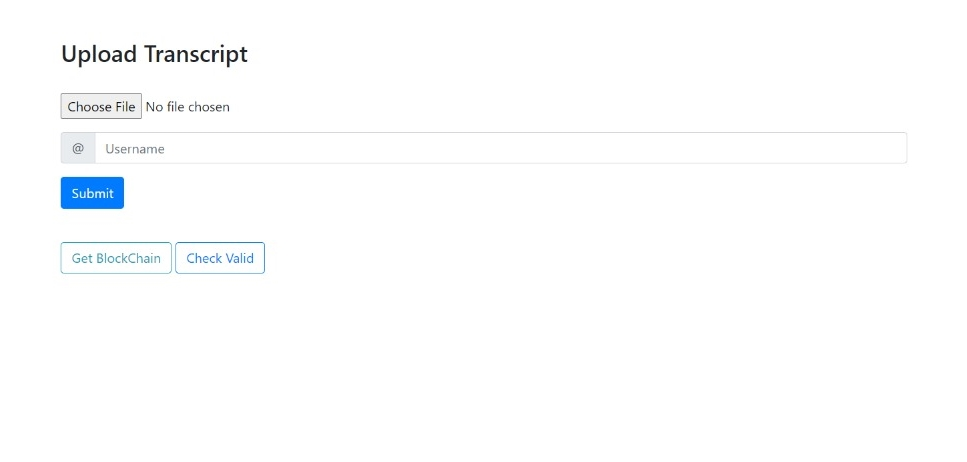
\includegraphics[scale=0.47]{images/upload_page.jpeg}\\[0.5cm]
    \caption{Upload Page Design}
    \label{fig:my_label}
\end{figure}

\begin{figure}[H]
    \centering
    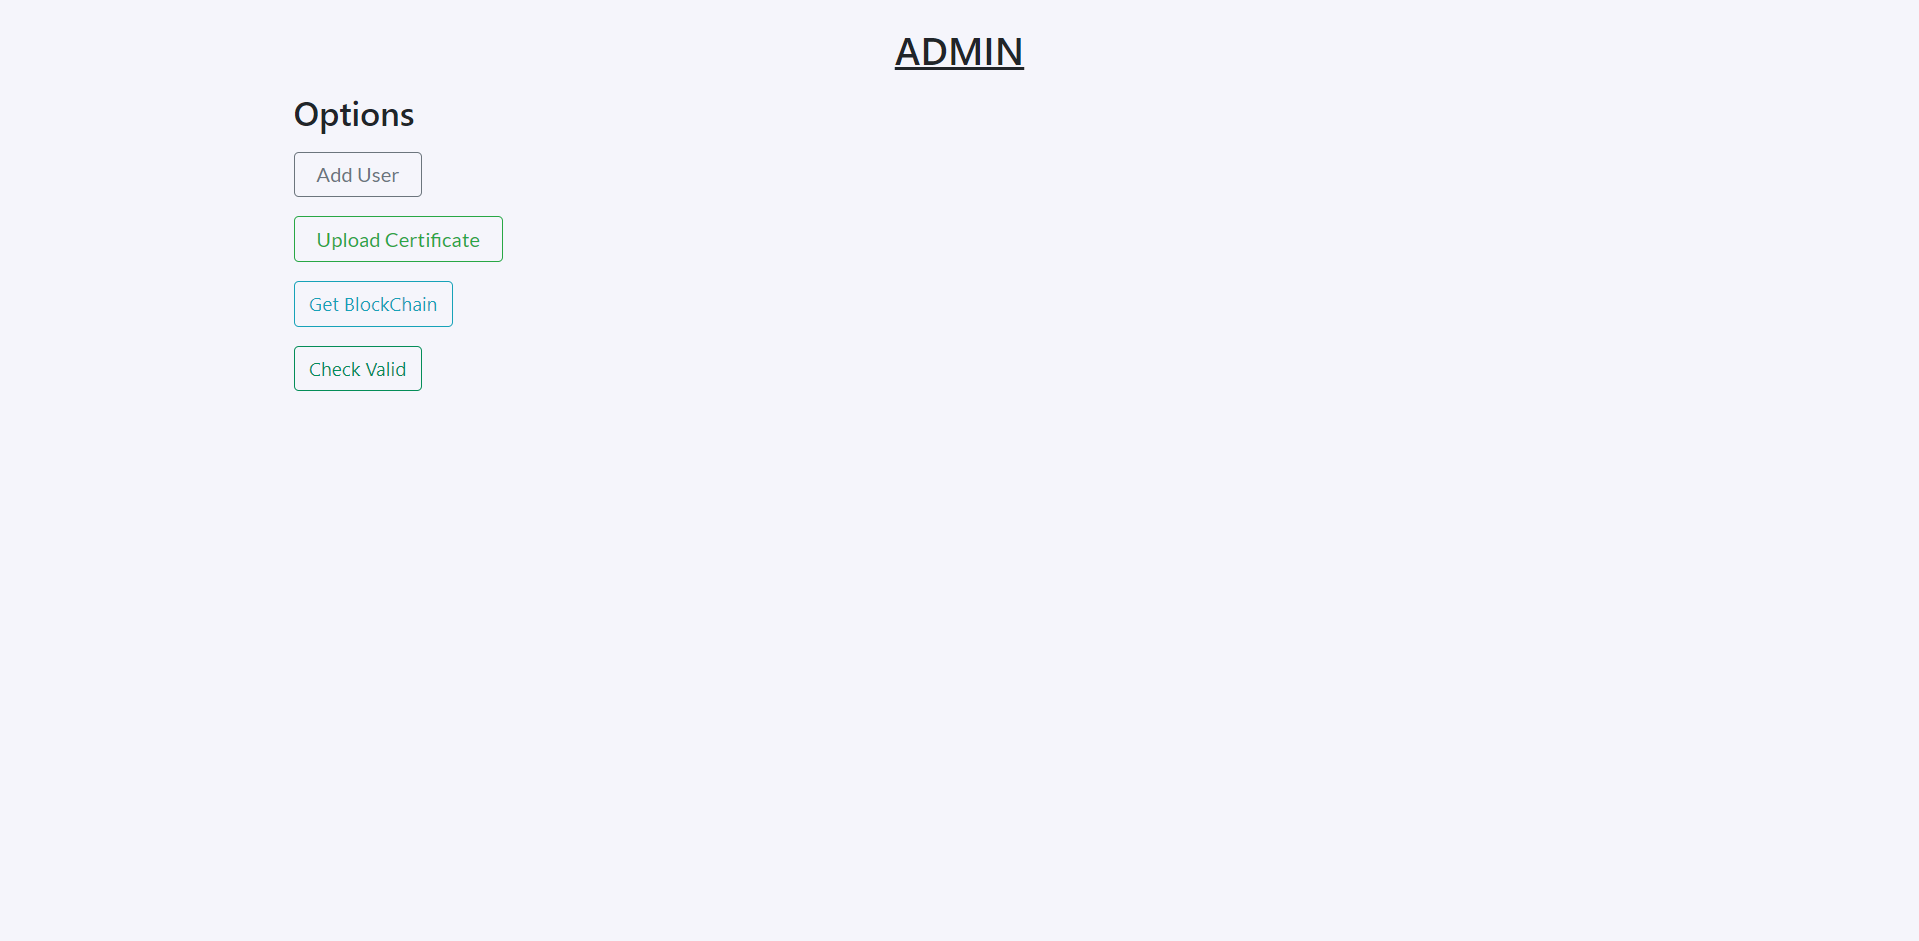
\includegraphics[scale=0.32]{images/Admin Page.png}\\[0.5cm]
    \caption{Admin Page}
    \label{fig:Admin Page}
\end{figure}

\begin{figure}[H]
    \centering
    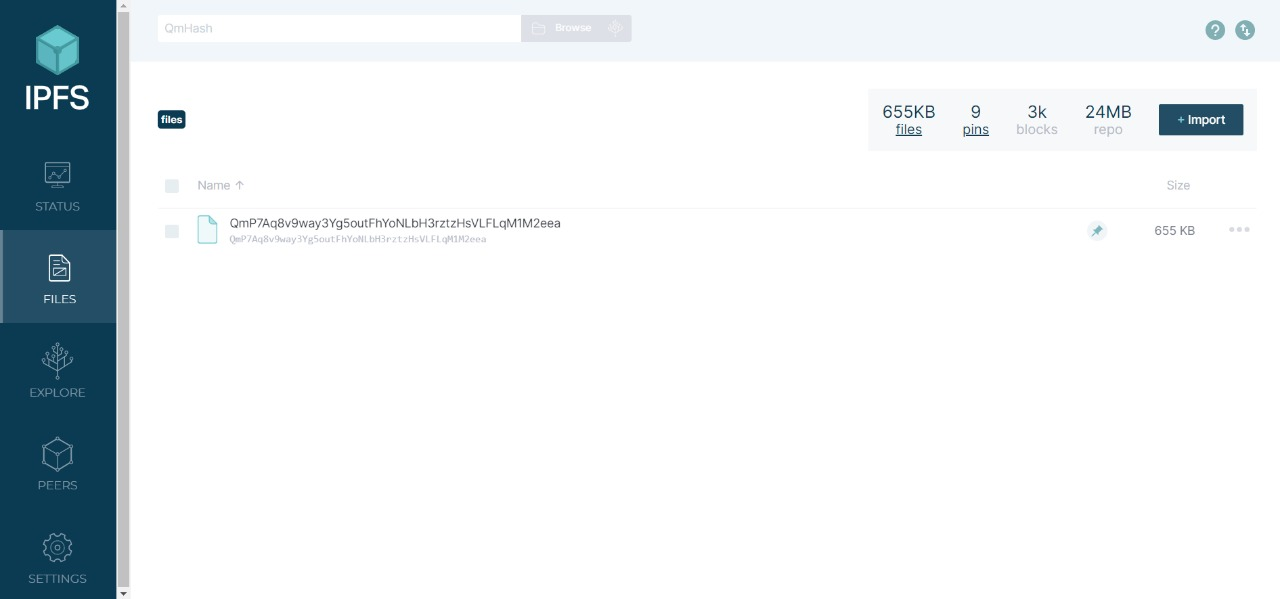
\includegraphics[scale=0.37]{images/ipfs-UI.jpeg}\\[0.5cm]
    \caption{IPFS Design}
    \label{fig:my_label}
\end{figure}
\subsection{Back Ends Representation (Database to be used )}
We have used the SQL Database and Flask for our project. Because SQL Database is used for having database of students.
Main Fields Included:
\begin{itemize}
    \item Name
    \item CRN
    \item Email
    \item Password
    \item ListOfBlocks
    \item EncryptPrivateKey
\end{itemize}
\subsubsection{Snapshots of Database Tables with brief description}
\begin{itemize}
    \item Name of the Student is of datatype text 
    \item Class Roll No. of the student is of datatype text and it is a primary key.
    \item Email of the student is of datatype text 
    \item Password of the student through which a student can login to view his/her certificates. It is of datatype text.
    \item ListOfBlocks: Indexes of the blocks in the block-chain having the hashes of the files uploaded on IPFS. It is of datatype text.w
    \item EncryptPrivateKey: Private Key which can be used for encrypting the file and decrypting the file that has been uploaded on IPFS.
\end{itemize}
\begin{longtable}{| >{\centering\arraybackslash}p{1.8cm} | >{\centering\arraybackslash}p{5.3cm} | >{\centering\arraybackslash}p{1.7cm} | >{\centering\arraybackslash}p{2cm} | >{\centering\arraybackslash}p{5.8cm} | >{\centering\arraybackslash}p{2cm} | >{\centering\arraybackslash}p{5cm} |}
    % \hline
\caption{Blockchain Database}


\label{table:table2} \\
\hline
        \textbf{Chain} \\ \hline
    1, 2  \\ \hline
    3, 4  \\ \hline
    
\end{longtable}
\begin{landscape}
\begin{longtable}{| >{\centering\arraybackslash}p{1.8cm} | >{\centering\arraybackslash}p{5.3cm} | >{\centering\arraybackslash}p{1.7cm} | >{\centering\arraybackslash}p{2cm} | >{\centering\arraybackslash}p{5.8cm} | >{\centering\arraybackslash}p{2cm} | >{\centering\arraybackslash}p{5cm} |}
    % \hline
\caption{Student Database}


\label{table:table1} \\
\hline
        \textbf{Name} & \textbf{Email} & \textbf{Username} & \textbf{Password} & \textbf{Encryption Key} & \textbf{List of Blocks} & \textbf{Hash} \\ \hline
    Vrishti Gupta & ivrishtigupta@gmail.com & 1915086 & vrishti123 & $07eVh2QgGdZeMqOM8FQCw$ & 2,5 & 6d8ace04726c183856a 0fcbc17b65cc f5bbfbad5afa1d3 3a2e0acda487267281 \\ \hline
    Priyanka Jhamb & priyankajhamb73@gmail.com & 1915103 & priyanka123 & $07eVh2QgGdZeMqOM8FQCw$ & 3,6 & 6d8ace04726c183856 a0fcbc17b65cc f5bbfbad5afa1d3 3a2e0acda487267281 \\ \hline
    Amanjot Singh & amanjots726@gmail.com & 1915105 & amanjot123 & $07eVh2QgGdZeMqOM8FQCw$ & 4,7 & 6d8ace04726c183856 a0fcbc17b65cc f5bbfbad5afa1d3 3a2e0acda487267281 \\ \hline
    
\end{longtable}
\end{landscape}


% \begin{table}[h!]
% \centering
% \caption{Keywords matched for search}
% \label{table:table1}
% \begin{tblr}{| >{\centering\arraybackslash}p{8cm} | >{\centering\arraybackslash}p{8cm} |}
%     \hline
%     \textbf{Classification} & \textbf{Keywords} \\
%     \hline
%     Target Population: Elderly & “Older adult” OR “older people” OR elderly OR elder OR senior OR aged OR 60-plus \\ [0.5cm] \hline 
%     Outcome: Human Activity Recognition & monitor* OR detection OR recognition \\ [0.5cm] \hline 
%     Specification: Daily Life Activities & walk* OR sit* OR stand* OR fall* \\ [0.5cm] \hline
%     Techniques: Activity recognition & Activity recognition techniques  \\ [0.5cm] \hline
%     Materials: Vision based or wearable sensors & Wearable OR vision-based OR sensors OR monitor* \\ [0.5cm] \hline
% \end{tblr}
% % \end{adjustwidth}
% \end{table}